\section{Diagrama de Use Case}

O diagrama de \textit{use case} é feito para se perceber as funcionalidades do sistema. Este, representa a interação entre um utilizador e o sistema. Com a elaboração destes, conseguiu-se perceber a unidade de um trabalho significante. Cada caso dos que serão apresentados na imagem seguinte, descreve a funcionalidade que irá ser construída no sistema proposto.

Importa salientar que com este diagrama, não se pretende que definir como o software deverá ser construído, mas sim como se deve comportar quando estiver pronto.

O desenvolvimento de um \textit{software} é algo bastante complexo, e o desenvolvimento dos diagramas de \textit{use case} descrevem uma "fatia" do que o \textit{software} deverá oferecer.

Estes, serão também os mais indicados para o cliente final visualizar, porque são construídos com linguagem natural, facilmente percetível por qualquer pessoa. \\


\begin{figure}[H]
\centerline{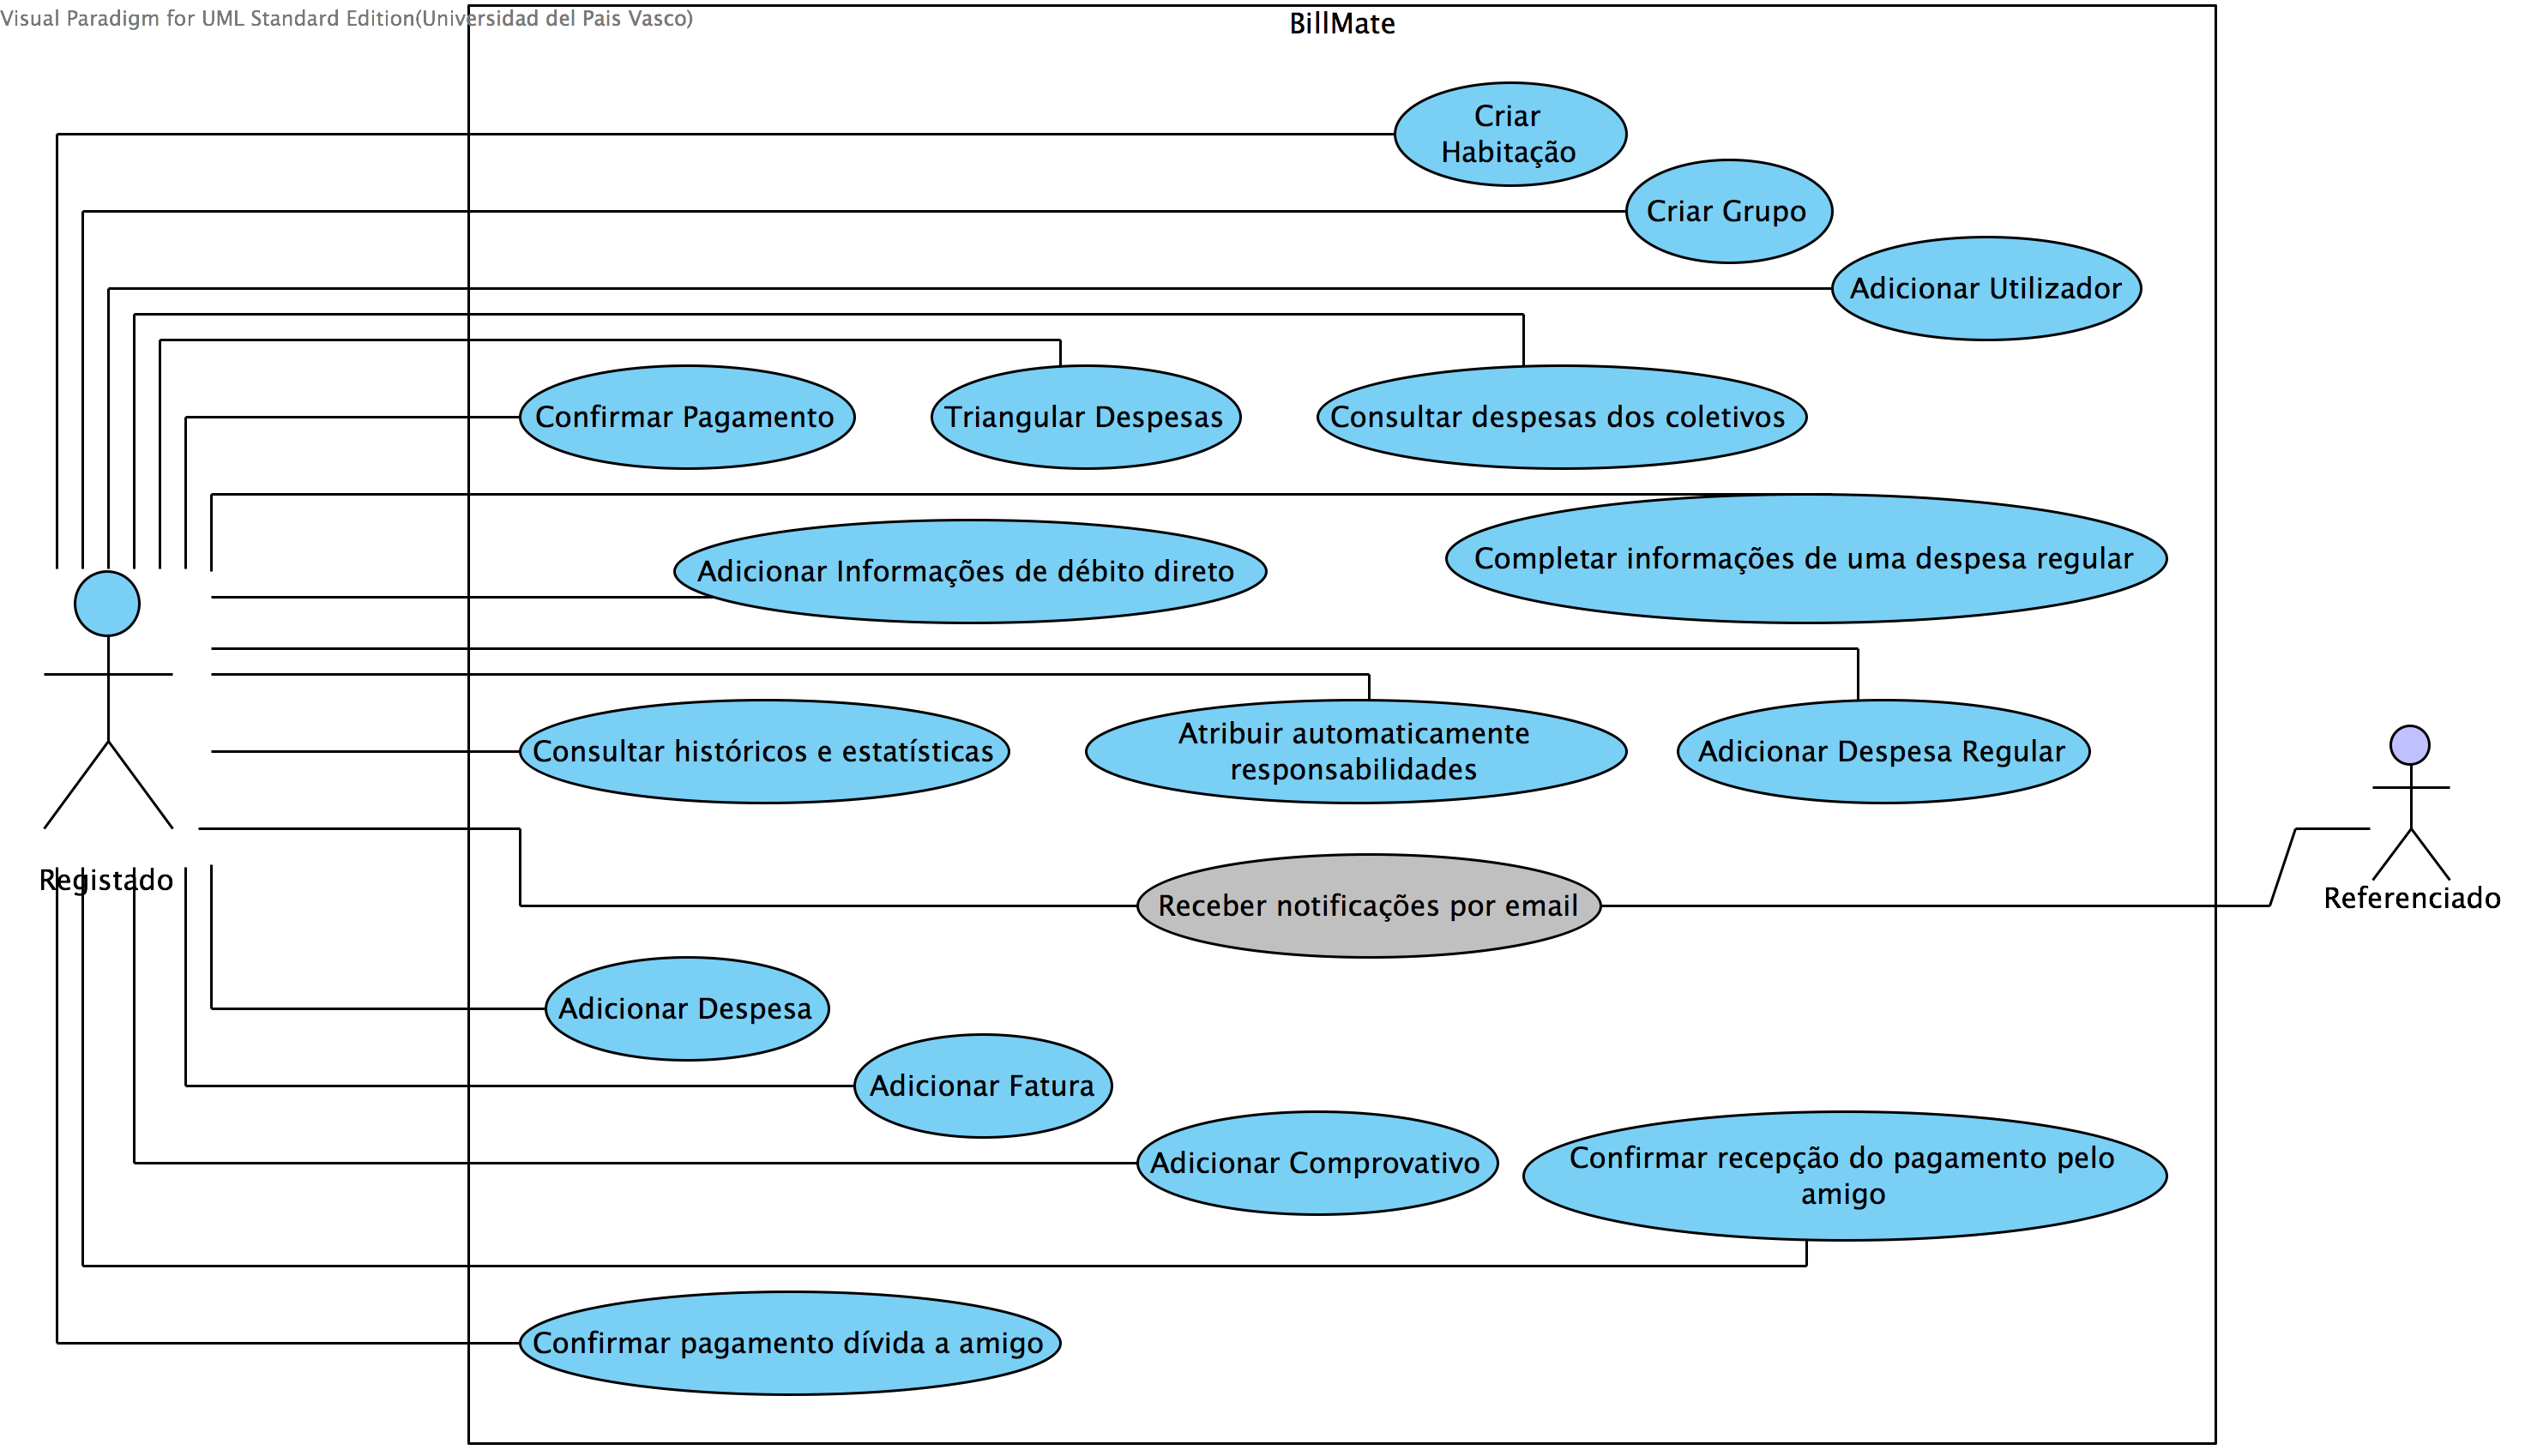
\includegraphics[width=1\textwidth]{images/modeling/useCase}}
\caption{Diagrama de use case}
\end{figure}
